%!TEX root = ../thesis.tex
%*******************************************************************************
%***************************** Fourth Chapter **********************************
%*******************************************************************************
\chapter{Results}

% **************************** Define Graphics Path **************************
\graphicspath{{Chapter4/Figs/}}


\section{Comparison between genetically encoded fluorescent proteins}

%Assume that I have explained in Backgrounds or Methods:
%	* binary expression systems
%	* genetically encoded fluorescent proteins
%	* ratiometric imaging


As explained in the previous chapters, in order to do ratiometric imaging, it is needed to use two
fluorescent proteins with sufficiently different excitation and emission spectra, and both FPs need
to be expressed in the same cells, or at least the same areas. One of the FPs has to be a calcium
indicator and the other one has to be calcium-independent FP.


For the calcium indicator, we have chosen the GCaMP6 family of indicators
\citep{nakai2001high,chen2013ultrasensitive}. More specifically, the GCaMP6s and GCaMP6f
indicators, because they are the latest published and brightest members of the family, have some
of the largest dynamic ranges of all GECIs, and are the de facto standard calcium indicators
\citep{lin2016genetically}.


For the calcium-independent FP, we identified three candidates, all in the orange-red part of the
visible light spectrum: mRFP1 \citep{campbell2002monomeric}, tdTomato \citep{shaner2004improved},
and mScarlet \citep{bindels2017mscarlet}. These candidate FPs were tested \textit{in vivo} by
crossing transgenic \textit{Drosophila} lines, UAS lines expressing the FPs and GAL4 lines targeting
specific cells, to achieve very targeted, very sparse expression of the FPs.

Each experiment consisted of recording at \SI{20}{\hertz} the unrestrained behaviour of a single
larva under a cover slip, as described in the Methods chapter.

\begin{figure}
	\centering
	\begin{subfigure}[b]{0.3\textwidth}
		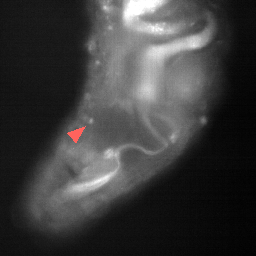
\includegraphics[width=\textwidth]{mRFP_full}
		\caption{mRFP}
		\label{fig:mrfp}
	\end{subfigure}
	\quad%
	\begin{subfigure}[b]{0.3\textwidth}
		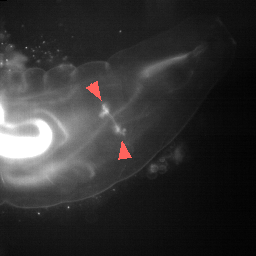
\includegraphics[width=\textwidth]{tdTomato_full}
		\caption{tdTomato}
		\label{fig:tdtomato}
	\end{subfigure}
	\quad%
	\begin{subfigure}[b]{0.3\textwidth}
		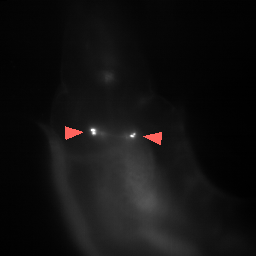
\includegraphics[width=\textwidth]{mScarlet_full}
		\caption{mScarlet}
		\label{fig:mscarlet}
	\end{subfigure}
	\caption{Expression pattern}
	\label{fig:expression_pattern}
\end{figure}

Figure~\ref{fig:expression_pattern} shows the expression pattern of the FPs,
Figure~\ref{fig:somas_projs} shows the somas and projections of the targeted cells,
and Figure~\ref{fig:timeseries} shows a comparison of the mean pixel values of the regions of interest
and the autofluorescence from the three FPs.

\begin{figure}
	\centering
	\begin{subfigure}[b]{0.3\textwidth}
		
\includegraphics[width=0.48\textwidth]{mRFP_1}
		
\includegraphics[width=0.48\textwidth]{mRFP_2} \\[2pt]
		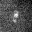
\includegraphics[width=0.48\textwidth]{mRFP_3}
		
\includegraphics[width=0.48\textwidth]{mRFP_4}
		\caption{mRFP somas}
		\label{fig:mrfp_somas}
	\end{subfigure}
	\quad%
	\begin{subfigure}[b]{0.3\textwidth}
		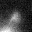
\includegraphics[width=0.48\textwidth]{tdTomato_1}
		
\includegraphics[width=0.48\textwidth]{tdTomato_2} \\[2pt]
		
\includegraphics[width=0.48\textwidth]{tdTomato_3}
		
\includegraphics[width=0.48\textwidth]{tdTomato_4}
		\caption{tdTomato somas}
		\label{fig:tdtomato_somas}
	\end{subfigure}
	\quad%
	\begin{subfigure}[b]{0.3\textwidth}
		
\includegraphics[width=0.48\textwidth]{mScarlet_1}
		
\includegraphics[width=0.48\textwidth]{mScarlet_2} \\[2pt]
		
\includegraphics[width=0.48\textwidth]{mScarlet_3}
		
\includegraphics[width=0.48\textwidth]{mScarlet_4}
		\caption{mScarlet somas}
		\label{fig:mscarlet_somas}
	\end{subfigure}

	\vspace{20pt}

	\begin{subfigure}[b]{0.3\textwidth}
		\centering
		
\includegraphics[width=0.57\textwidth]{tdTomato_projections_1} \\[2pt]
		
\includegraphics[width=0.57\textwidth]{tdTomato_projections_2}
		\caption{tdTomato projections}
		\label{fig:tdtomato_projections}
	\end{subfigure}
	\quad%
	\begin{subfigure}[b]{0.3\textwidth}
		\centering
		
\includegraphics[width=0.48\textwidth]{mScarlet_projections_1} \\[2pt]
		
\includegraphics[width=0.48\textwidth]{mScarlet_projections_2}
		\caption{mScarlet projections}
		\label{fig:mscarlet_projections}
	\end{subfigure}

	\caption{Somas and Projections}
	\label{fig:somas_projs}
\end{figure}

\begin{figure}
	\centering
	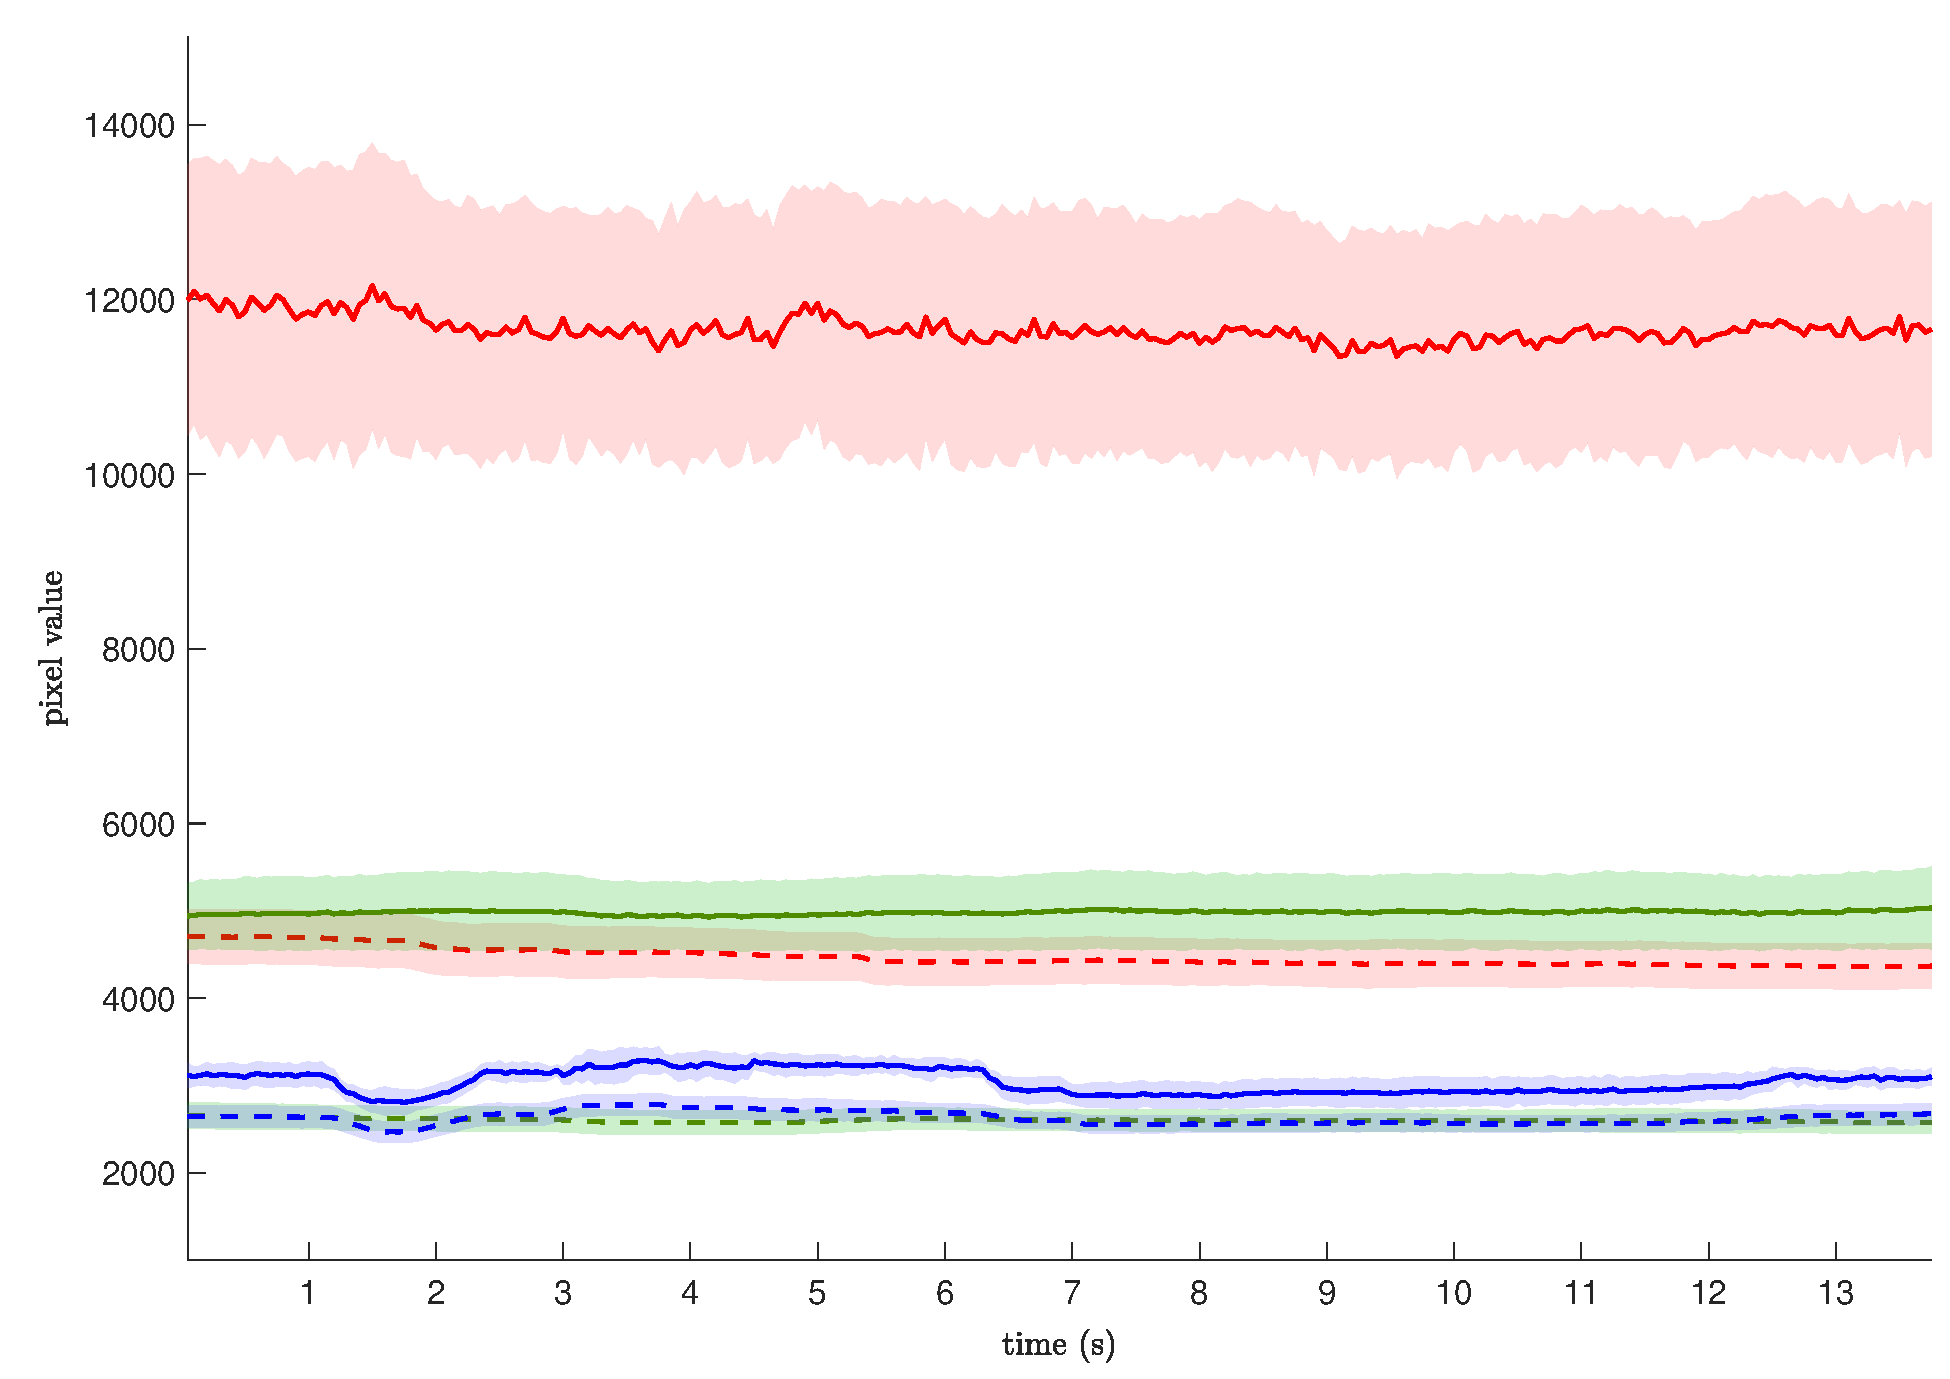
\includegraphics[width=0.7\textwidth]{intensity_timeseries}
	\caption{
		Timeseries of mean pixel value of regions of interest and autofluorescence
	}
	Blue --- mRFP, green --- tdTomato, red --- mScarlet. Solid --- regions of interest,
	dashed --- autofluorescence. Filled areas --- standard deviation of the pixel values in region
	of interest.
	\label{fig:timeseries}
\end{figure}

The FPs were compared based on a few criteria: expression pattern, difference between fluorescence
in the regions of interest and autofluorescence, and dynamic range.

\textbf{Talk about each criteria and how the FPs meet them (or don't)...}

It is clear from the data that mScarlet seems to best among the three FPs, according to all
criteria.

\textbf{Anything else?}

Something that needs to be mentioned is that the light filters were not changed in-between
experiments. And since the filters were optimised for imaging with tdTomato, it may be
possible to significantly improve the signals from mRFP and mScarlet by changing the filters to
adjust the cut-on and cut-off wavelengths.
